\chapter{Progettazione}
\label{cap:progettazione}

La progettazione del sistema è un passo fondamentale per lo sviluppo di un sistema software.\\
In questo capitolo verranno descritte le scelte progettuali effettuate per la progettazione del sistema, in particolare per lo sviluppo del database, il frontend, il backend e l'integrazione con Azure Media Services.\\
\section{Progettazione del database}
La progettazione del database è stata effettuata sulla base dei requisiti funzionali e non funzionali individuati in fase di analisi.\\
Il database è stato progettato per memorizzare i dati relativi agli eventi, video e utenti.\\
Per la sua progettazione è stato utilizzato il framework Entity Framework Core, che permette di definire il modello del database utilizzando classi e proprietà direttamente dal codice. Non è stato necessario scrivere codice SQL per la creazione del database, ma è stato sufficiente definire le classi e le proprietà dei modelli e successivamente eseguire le migrazioni per aggiornare il database.\\
\subsection{Modello del database}
Il database è composto da tre tabelle: Event, Video e User.\\
La tabella Event contiene i dati relativi agli eventi, come l'id, il titolo, l'id dell'user che l'ha creato, la data di inizio e di fine e l'URL alla thumbnail; la tabella Video contiene i dati relativi ai video, come l'id, il titolo, l'URL alla thumbnail, l'URL al video e l'id dell'evento a cui appartiene; la tabella User contiene i dati relativi agli utenti, come l'id e il nome;
\begin{figure}[H] 
    \centering 
    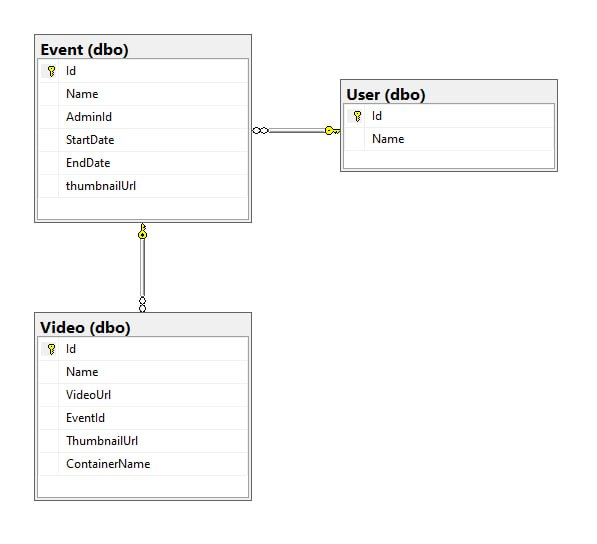
\includegraphics[scale=0.5]{diagrammi/database.png} 
    \caption{Diagramma del database}
\end{figure}
\section{Progettazione del frontend}
La progettazione del frontend è sviluppata sulla base dell'utilizzo di React come libreria principale per lo sviluppo dell'interfaccia utente.
%  Verranno illustrati i principi di progettazione di React, come la creazione di componenti riutilizzabili, la gestione dello stato dell'applicazione e la definizione delle rotte per la navigazione. Saranno presentati anche i diagrammi dell'architettura del frontend, mostrando come i componenti si integrano per creare un'esperienza utente coerente.
\subsection{Architettura del frontend}
Il frontend è sviluppato utilizzando un template disposto dall'azienda, che utilizza il design pattern Container-Presenter, è composto da due componenti principali: il Container e il Presenter.
Il primo è responsabile della gestione dello stato dell'applicazione, dell'interazione con i dati e della logica di business, si occupa di recuperare i dati, gestire gli eventi, effettuare chiamate API e gestire lo stato globale dell'applicazione; il secondo invece, è responsabile dell'aspetto visuale e dell'interfaccia utente, riceve i dati e le funzioni dai Container e si occupa di renderizzare l'interfaccia utente in base ai dati ricevuti.\\
La comunicazione tra i due avviene tramite le props, in quanto il Container passa i dati al Presenter tramite props, mentre il Presenter invia le informazioni tramite callback fornite dal Container.\\
\subsection{Diagrammi dell'architettura del frontend}
\subsubsection{Diagramma dell'architettura}
\begin{figure}[!h] 
    \centering 
    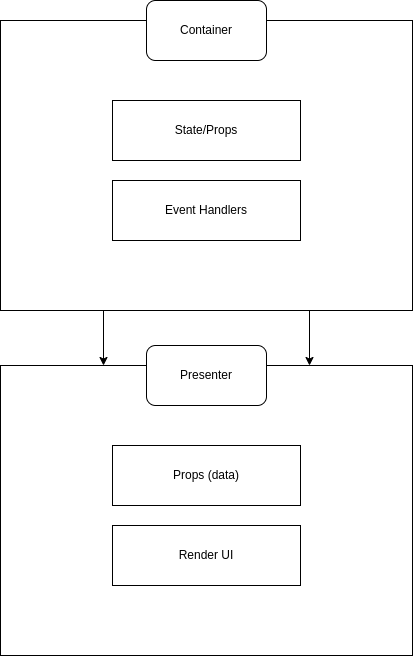
\includegraphics[scale=0.5]{diagrammi/frontend.drawio.png} 
    \caption{Diagramma design pattern Container-Presenter}
\end{figure}
\clearpage
\section{Progettazione del backend}
La progettazione del backend è sviluppata sulla base dell'utilizzo del linguaggio di programmazione C\texttt{\#} e del framework ASP.NET Core.\\
\subsection{Architettura del backend}
Il backend è sviluppato utilizzando un template disposto dall'azienda, che utilizza una separazione delle componenti in layer distinti, dove ognuno ha un compito specifico.\\
Il template è composto da tre layer fondamentali: API, Core e Data; il primo è responsabile della comunicazione con il frontend, il secondo è responsabile della gestione dello stato dell'applicazione e il terzo è responsabile della comunicazione con il database.\\
\subsubsection{API}
È responsabile della comunicazione con il frontend, è composto da due parti: i controller e i DTO. Il primo ha il compito di gestire le richieste HTTP provenienti dal frontend e coordinare le azioni richieste per soddisfarle: quando un controller riceve una richiesta, estrae i dati necessari dalla richiesta e interagisce con i layer Core per fornire una risposta al Client. 
Il secondo ha il compito di definire la struttura dei dati che vengono trasferiti tra il frontend e il backend durante la chiamata, in modo da consentire una comunicazione standardizzata e senza ambiguità. I DTO possono includere solo i campi necessari per soddisfare una certa richiesta, così facendo, riducono il trasferimento di dati inutili e rendono la comunicazione più veloce; oltre a ciò, sono utilizzati anche per la validazione dei dati, garantendo che i dati ricevuti dal frontend siano validi.\\
\subsubsection{Core}
Il layer Core è responsabile della gestione dello stato dell'applicazione. Riceve le richieste dal layer API e le elabora, interagendo con il layer Data per ottenere i dati necessari; è composto da due parti: i models e i service. I models rappresentano la struttura dei dati che vengono utilizzati dall'applicazione per effettuare le operazioni richieste; i service, invece, gestiscono la logica dell'applicazione, contengono i metodi che vengono chiamati dai controller, che eseguono operazioni con i servizi esterni e con il layer Data.\\
\subsubsection{Data}
Il layer Data è responsabile dell'accesso ai dati, è composto da tre parti: Context, Entity e Provider. Il primo ha il compito di gestire la connessione con il database, definisce la struttura del database e fornisce i metodi per accedervi; il secondo ha il compito di definire la struttura dei dati che vengono salvati nel database; il terzo ha il compito di gestire la comunicazione con il database, fornisce i metodi per accedere ai dati per effettuare le operazioni di lettura e scrittura.\\
\subsection{Diagrammi dell'architettura del backend}
\subsubsection{Diagramma dell'architettura}
\begin{figure}[H] 
    \centering 
    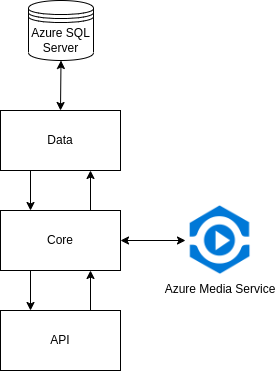
\includegraphics[scale=0.5]{diagrammi/backend.png} 
    \caption{Diagramma architettura del backend}
\end{figure}
\section{Integrazione con Azure}
Azure è una piattaforma cloud proprietaria di Microsoft che offre vari servizi.
La WebApp è integrata con Azure per la gestione del database, gestione dei video e per la distribuzione dell'applicazione, sono utilizzati i seguenti servizi: SQL Server, Azure Media Service e Azure App Service.\\
\subsection{Azure SQL Server}
Il progetto integra un database SQL ospitato su Azure SQL Server, che permette di gestire il database in maniera semplice e veloce, senza dover gestire l'infrastruttura. Il collegamento al database è gestito dal layer Data del backend, che utilizza Entity Framework Core per la gestione del database.\\
\subsection{Azure Media Service}
Il progetto utilizza Azure Media Service per la gestione dei video, in particolare per la codifica, l'archiviazione e la distribuzione dei video. Il collegamento ad Azure Media Service è gestito dal layer Core del backend, che utilizza il package NuGet Microsoft.Azure.Management.Media per la gestione dei video.\\
\subsubsection{Codifica}
Per lo sviluppo di questo PoC è stato deciso di codificare i video in H.264 e utilizzando il preset Adaptive Streaming, che permette di codificare il video in diversi formati e risoluzioni, in modo da adattarsi alla qualità della rete e al dispositivo utilizzato. Sono state scelte queste impostazioni che permettono di ottenere un video di risoluzione massima pari a 1080p.\\
\subsubsection{Archiviazione}
Quando un video termina la codifica, viene archiviato in un container di Azure Media Service, che permette il salvataggio dei vari file video, della thumbnail, dei metadati e del manifest.\\
\subsubsection{Distribuzione}
Una volta archiviato, il video viene distribuito tramite Streaming Endpoint, che creano un Url al manifest del video e all'immagine di thumbnail, che vengono poi salvati nel database tramite apposite API.\\
\subsubsection{Azure App Service}
Sia il modulo FrontEnd che il modulo del Backend vengono distribuiti attraverso Azure App Service, vengono inizializzati tramite l'apposita funzione di Visual Studio 2022.\\ 